
\section{Sistema di gestione}

\begin{figure}[H]
    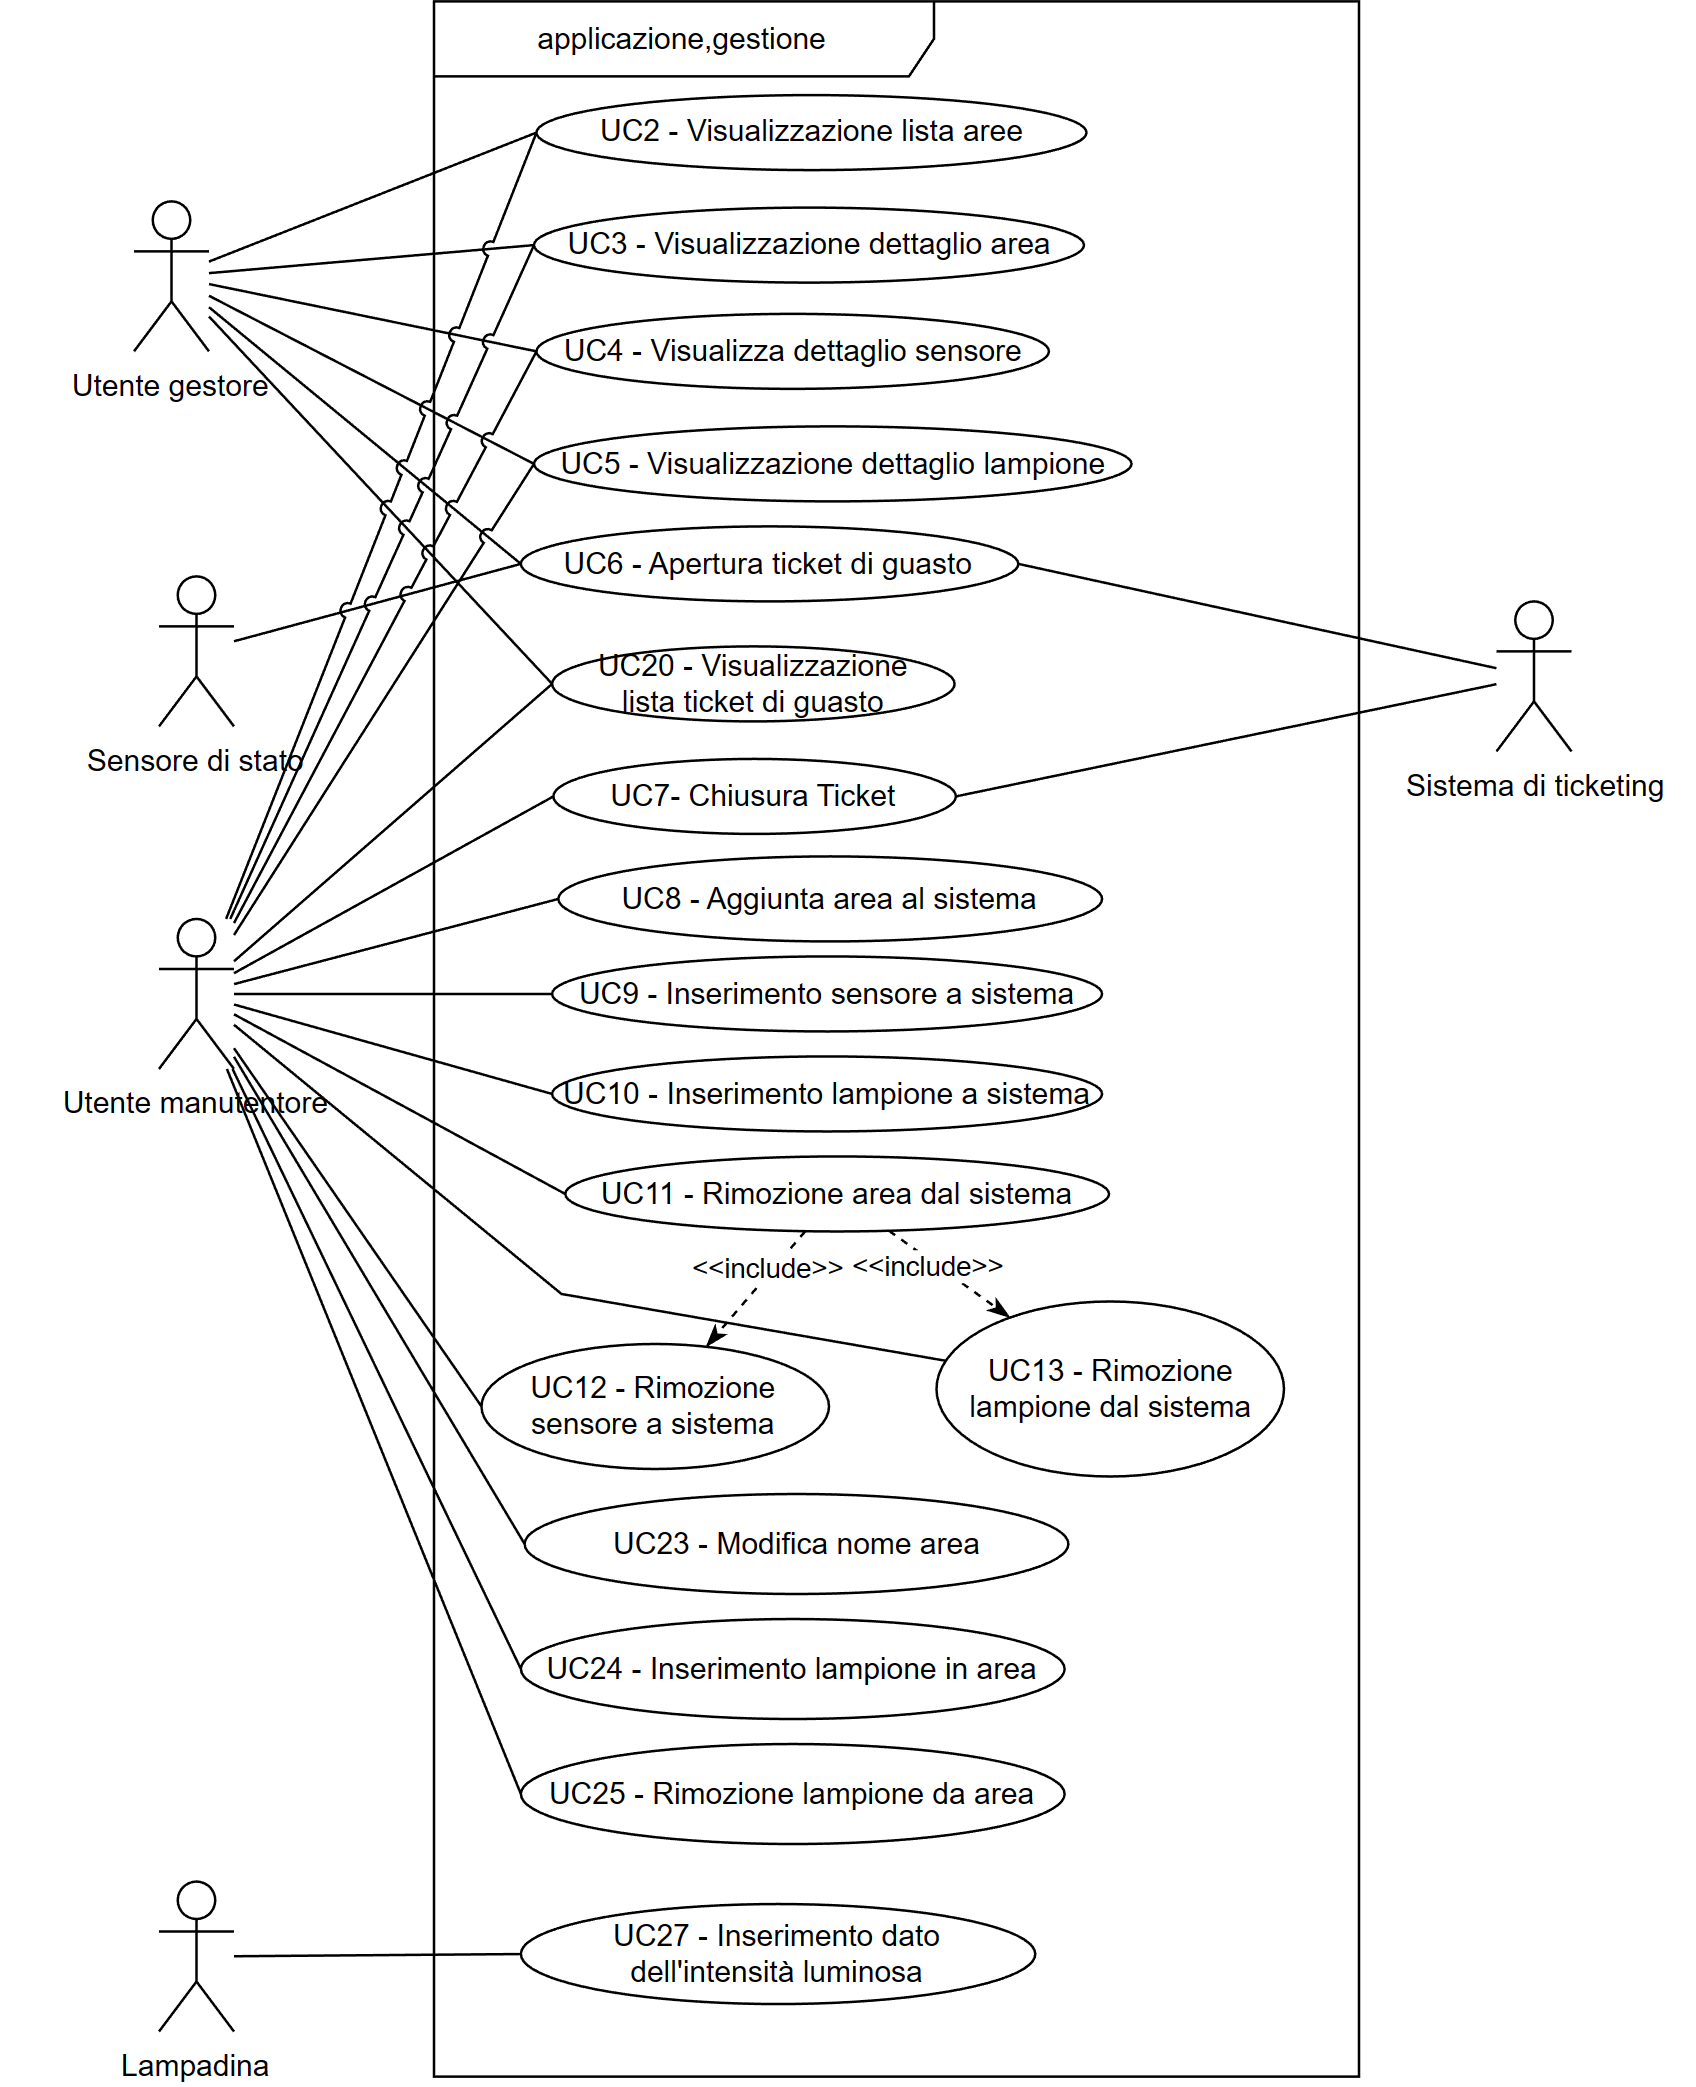
\includegraphics[width=\textwidth]{contenuti/img/casi_uso_grafici-applicazione,gestione.png}
    \caption{Parte relativa alla gestione dell'applicazione}
    \label{fig:gestione}
\end{figure}

\subsection{I casi d'uso descritti}

\begin{itemize}
    \item \hyperref[uc:02]{UC02 Visualizzazione lista aree}
    \item \hyperref[uc:03]{UC03 Visualizzazione dettaglio area}
    \item \hyperref[uc:04]{UC04 Visualizzazione dettaglio sensore}
    \item \hyperref[uc:05]{UC05 Visualizzazione dettaglio lampione}
    \item \hyperref[uc:06]{UC06 Apertura ticket di guasto}
    \item \hyperref[uc:07]{UC07 Chiusura ticket}
    \item \hyperref[uc:08]{UC08 Aggiunta area al sistema}
    \item \hyperref[uc:09]{UC09 Inserimento sensore a sistema}
    \item \hyperref[uc:10]{UC10 Inserimento lampione a sistema}
    \item \hyperref[uc:11]{UC11 Rimozione area dal sistema}
    \item \hyperref[uc:12]{UC12 Rimozione sensore dal sistema}
    \item \hyperref[uc:13]{UC13 Rimozione lampione dal sistema}
    \item \hyperref[uc:26]{UC26 Inserimento dato dell'intensità luminosa}
\end{itemize}